\section{COTH Hyperbolic Cotangent Function}

\subsection{Usage}

Computes the hyperbolic cotangent of the argument.
The syntax for its use is
\begin{verbatim}
   y = coth(x)
\end{verbatim}
\subsection{Function Internals}

The \verb|coth| function is computed from the formula
\[
   \coth(x) = \frac{1}{\tanh(x)}
\]
\subsection{Examples}

Here is a simple plot of the hyperbolic cotangent function
\begin{verbatim}
--> x1 = -pi+.01:.01:-.01;
--> x2 = .01:.01:pi-.01;
--> plot(x1,coth(x1),x2,coth(x2)); grid('on');
\end{verbatim}


\centerline{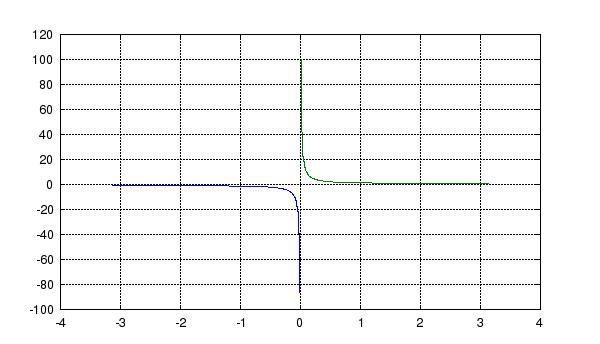
\includegraphics[width=8cm]{cothplot}}

